\chapter{Mise en Œuvre du Sprint 2 : Développement du Web Scraping et Preprocessing des Données}

\section{Introduction}

Dans le cadre du sprint 2, l'équipe s'est focalisée sur le développement du module de web scraping avec Selenium pour automatiser la collecte des commentaires sur Hespress, ainsi que sur la mise en place du prétraitement et nettoyage des données avec Pandas. Cette phase constitue le cœur opérationnel de notre application de détection de sentiments, établissant un pipeline robuste de collecte et de traitement des données nécessaires à l'analyse.

L'objectif principal de ce sprint était de créer un système automatisé de collecte de données capable d'extraire efficacement les commentaires du site Hespress en utilisant Selenium WebDriver, puis d'implémenter les algorithmes de preprocessing et de nettoyage des données avec Pandas pour préparer ces données à l'analyse de sentiments avec le modèle cardiffnlp/twitter-xlm-roberta-base-sentiment. De plus, l'initialisation de l'API de récupération des données a été mise en place pour permettre l'accès programmatique aux données collectées.

Cette phase s'appuie sur l'infrastructure technique établie lors du sprint 1 (configuration de l'environnement Next.js, FastAPI, Spring et authentification Keycloak) et constitue une étape cruciale pour alimenter le système d'analyse avec des données de qualité, nettoyées et structurées pour optimiser les performances du modèle de classification de sentiments.

\section{Backlog du Sprint 2}

Le développement de notre application de détection de sentiments des commentaires sur Hespress s'est structuré autour d'un backlog produit bien défini, comprenant plusieurs épopées et user stories. Le sprint 2 se concentre spécifiquement sur la collecte et le traitement des données avec Selenium et Pandas, ainsi que sur l'initialisation de l'API de récupération des données, étapes fondamentales pour l'efficacité du système d'analyse.

\subsection{Épopée 2 : Web Scraping et Traitement des Données}

Cette épopée couvre l'ensemble du pipeline de données, depuis la collecte automatisée avec Selenium jusqu'au preprocessing avancé des textes avec Pandas et l'API de récupération des données.

\subsubsection{User Story 2.1 : Développement du Web Scraping avec Selenium}

\textbf{En tant que} : système automatisé \\
\textbf{Je veux} : collecter automatiquement les commentaires du site Hespress en utilisant Selenium WebDriver \\
\textbf{Afin de} : disposer d'un flux continu de données pour l'analyse de sentiments

\textbf{Critères d'acceptation :}
\begin{itemize}
    \item Le système utilise Selenium WebDriver pour naviguer automatiquement sur le site Hespress
    \item Les commentaires sont extraits avec leurs métadonnées (date, article, auteur)
    \item Le scraping gère les éléments JavaScript dynamiques du site
    \item Les données collectées sont stockées dans une structure cohérente
    \item Le système gère les erreurs de connexion et les changements de structure du site
    \item Respect des limitations de taux pour éviter la surcharge du serveur
\end{itemize}

\subsubsection{User Story 2.2 : Prétraitement et Nettoyage des Données avec Pandas}

\textbf{En tant que} : système d'analyse \\
\textbf{Je veux} : nettoyer et préparer les données textuelles collectées en utilisant Pandas \\
\textbf{Afin d'} : optimiser la précision du modèle cardiffnlp/twitter-xlm-roberta-base-sentiment

\textbf{Critères d'acceptation :}
\begin{itemize}
    \item Utilisation de Pandas pour la manipulation et le nettoyage des données
    \item Les textes sont nettoyés (suppression des caractères spéciaux, HTML, etc.)
    \item La normalisation multilingue (arabe, français, darija) est appliquée
    \item Les doublons sont détectés et supprimés avec Pandas
    \item La tokenisation et la lemmatisation sont effectuées selon la langue
    \item Les textes trop courts ou non pertinents sont filtrés
    \item Les données sont formatées pour être compatibles avec le modèle de sentiment
\end{itemize}

\subsubsection{User Story 2.3 : Initialisation de l'API de Récupération des Données}

\textbf{En tant que} : développeur \\
\textbf{Je veux} : accéder aux données collectées et prétraitées via une API REST \\
\textbf{Afin de} : intégrer facilement les données dans le système d'analyse de sentiments

\textbf{Critères d'acceptation :}
\begin{itemize}
    \item Une API REST est développée pour accéder aux données collectées
    \item L'API permet la récupération des commentaires par date, article ou critères
    \item Les endpoints sont documentés et testés
    \item L'API s'intègre avec l'architecture FastAPI existante
    \item Les données retournées sont formatées en JSON
    \item Pagination et filtrage des résultats disponibles
\end{itemize}

\subsection{Sprint Plan}

Le plan de développement s'articule autour de quatre sprints principaux selon le plan de release défini :

\begin{itemize}
    \item \textbf{Sprint 1 :} Configuration de l'environnement de développement (Next.js, FastAPI, Spring) et mise en place de l'authentification via Keycloak
    \item \textbf{Sprint 2 :} Développement du module de web scraping avec Selenium, prétraitement et nettoyage des données avec Pandas, et initialisation de l'API de récupération des données
    \item \textbf{Sprint 3 :} Intégration du modèle d'analyse de sentiment (cardiffnlp/twitter-xlm-roberta-base-sentiment de Hugging Face) et démarrage du tableau de bord de visualisation
    \item \textbf{Sprint 4 :} Génération automatique des rapports d'analyse et phase complète de tests fonctionnels
\end{itemize}

Le sprint 2 constitue le pilier du pipeline de données, établissant les fondations technologiques avec Selenium pour la collecte automatisée et Pandas pour le traitement des commentaires d'Hespress, complétées par une API robuste pour l'accès aux données.

\section{Analyse et Conception}

\subsection{Description Textuelle}

Le développement du sprint 2 s'est organisé autour de trois axes technologiques majeurs, en parfaite cohérence avec l'architecture de l'application de détection de sentiments des commentaires sur Hespress :

\textbf{Développement du Module de Web Scraping avec Selenium :} L'équipe a conçu et implémenté un système robuste de collecte automatisée utilisant Selenium WebDriver pour naviguer sur le site Hespress. Ce module exploite les capacités de Selenium pour gérer les éléments JavaScript dynamiques, identifier précisément les sections de commentaires, et extraire les données textuelles avec leurs métadonnées associées (date, auteur, article source). Le système intègre des mécanismes avancés de gestion d'erreurs, de rotation des user agents, et de respect des délais pour éviter la détection anti-bot tout en maintenant une collecte efficace.

\textbf{Implémentation du Prétraitement et Nettoyage avec Pandas :} Un pipeline complet de preprocessing a été développé en exploitant les puissantes fonctionnalités de Pandas pour la manipulation et l'analyse des données. Ce système utilise les DataFrames Pandas pour structurer les données collectées, applique des techniques de nettoyage avancées (détection automatique de langue arabe, français, darija), normalise les caractères, supprime les balises HTML et les caractères spéciaux, et effectue une tokenisation adaptée aux spécificités linguistiques marocaines. Les algorithmes de détection de doublons et de filtrage de qualité exploitent les méthodes optimisées de Pandas pour traiter efficacement de gros volumes de données.

\textbf{Initialisation de l'API de Récupération des Données :} Une interface programmatique REST a été développée pour permettre l'accès structuré aux données collectées et prétraitées. Cette API, intégrée dans l'architecture FastAPI existante, propose des endpoints documentés pour la récupération des commentaires selon différents critères (date, article, sentiment), avec des fonctionnalités de pagination et de filtrage. L'API garantit la cohérence des données en format JSON et facilite l'intégration avec les composants d'analyse de sentiment qui seront développés lors du sprint 3.

\textbf{Optimisation des Performances et Intégration :} L'architecture a été optimisée pour traiter de gros volumes de données en exploitant les capacités vectorisées de Pandas et les techniques de parallélisation de Selenium. L'utilisation de pools de connexions et de mise en cache intelligente permet de maintenir des performances élevées même avec des milliers de commentaires à traiter. L'intégration avec PostgreSQL pour le stockage et Redis pour le cache assure une persistance robuste et des accès rapides aux données.

\textbf{Tests et Validation :} Des tests approfondis ont été menés pour valider la robustesse du scraping Selenium face aux changements de structure du site Hespress, ainsi que la qualité du preprocessing Pandas sur différents types de contenus textuels multilingues. Des métriques de qualité spécifiques ont été établies pour surveiller l'efficacité du pipeline de données et préparer l'intégration avec le modèle cardiffnlp/twitter-xlm-roberta-base-sentiment prévu pour le sprint 3.

\subsection{Diagramme de Cas d'Utilisation du Sprint 2}

\begin{figure}[H]
\centering
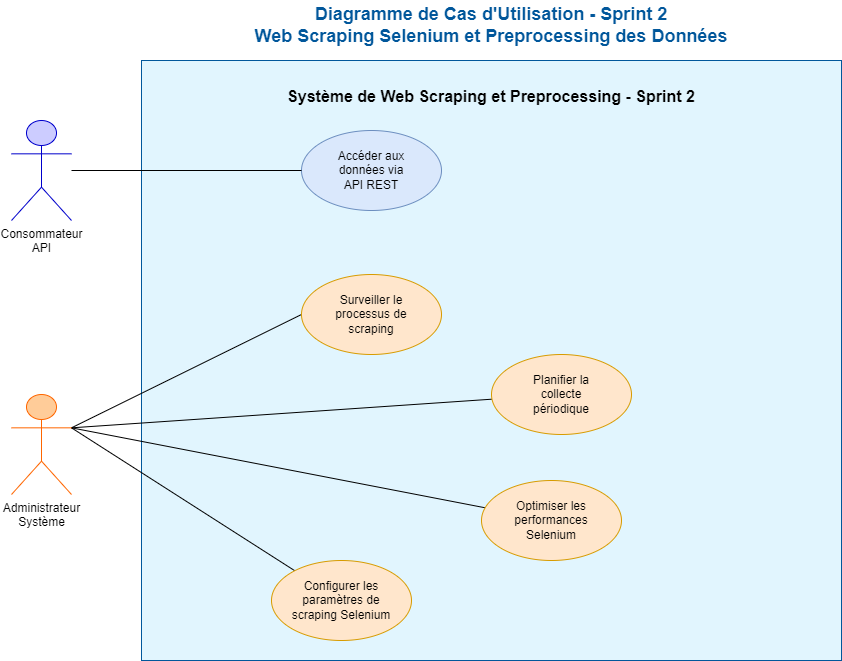
\includegraphics[width=0.8\textwidth]{assets/images/sprint2-usecase.png}
\caption{Diagramme de cas d'utilisation du sprint 2}
\label{fig:sprint2-usecase}
\end{figure}

Ce diagramme illustre les interactions entre le système de scraping Selenium, le module de preprocessing Pandas et l'API de récupération des données durant le sprint 2. Les cas d'utilisation se concentrent sur la collecte automatisée des commentaires, leur traitement avec Pandas, et l'exposition des données via l'API REST.

\subsection{Diagramme de Classe du Sprint 2}

\begin{figure}[H]
\centering
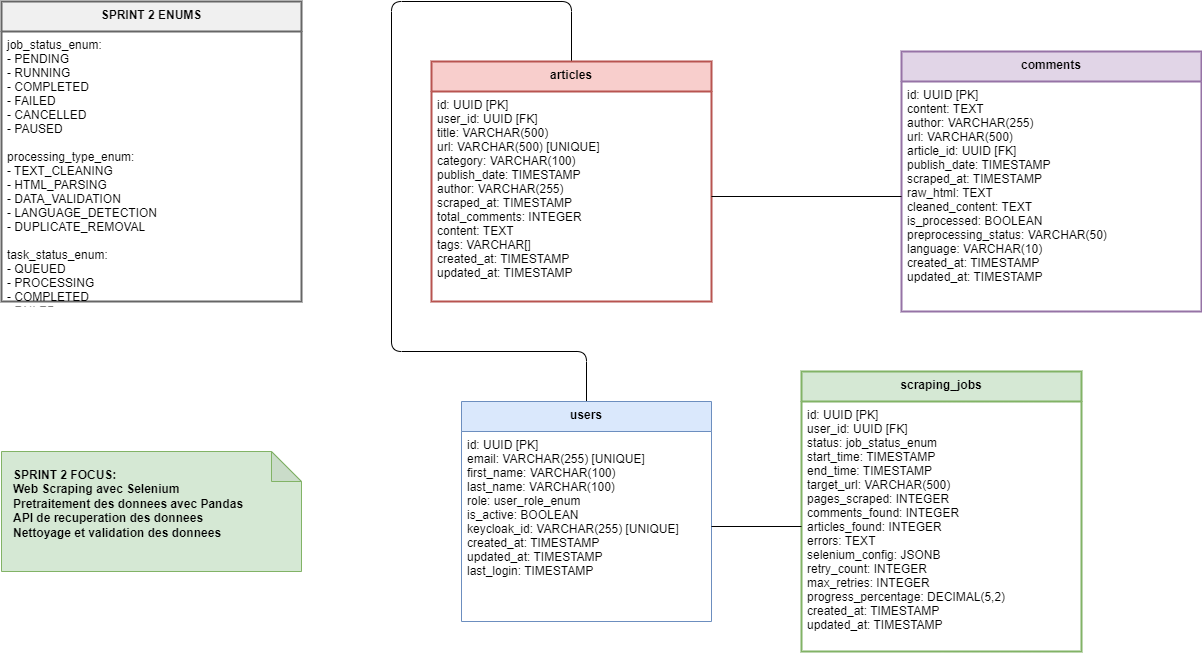
\includegraphics[width=0.9\textwidth]{assets/images/sprint2-class.png}
\caption{Diagramme de classe du sprint 2}
\label{fig:sprint2-class}
\end{figure}

L'architecture objet du sprint 2 met en évidence les nouvelles classes introduites : SeleniumWebScraper, CommentExtractor, PandasDataPreprocessor, TextNormalizer, et DataAPI. Ces classes forment le pipeline complet de collecte avec Selenium, de traitement avec Pandas, et d'exposition des données via l'API REST.

\subsection{Diagramme de Séquence du Pipeline de Données}

\begin{figure}[H]
\centering
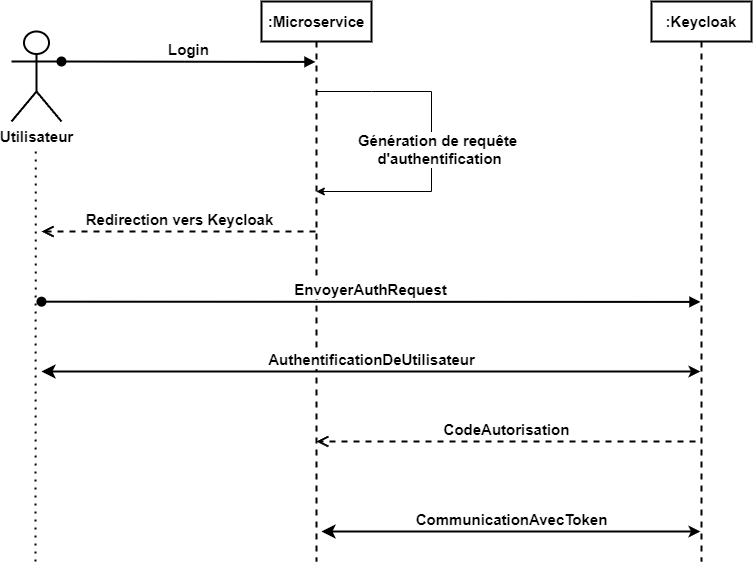
\includegraphics[width=0.9\textwidth]{assets/images/keycloak-seq.png}
\caption{Diagramme de séquence du processus de collecte et preprocessing}
\label{fig:data-pipeline-sequence}
\end{figure}

Ce diagramme détaille le flux d'exécution depuis le déclenchement de la collecte jusqu'au stockage des données preprocessées. Il montre l'orchestration entre le module de scraping Selenium, les algorithmes de preprocessing, et la base de données pour constituer un pipeline de données robuste.

\subsection{Architecture du Pipeline de Données}

\begin{figure}[H]
\centering
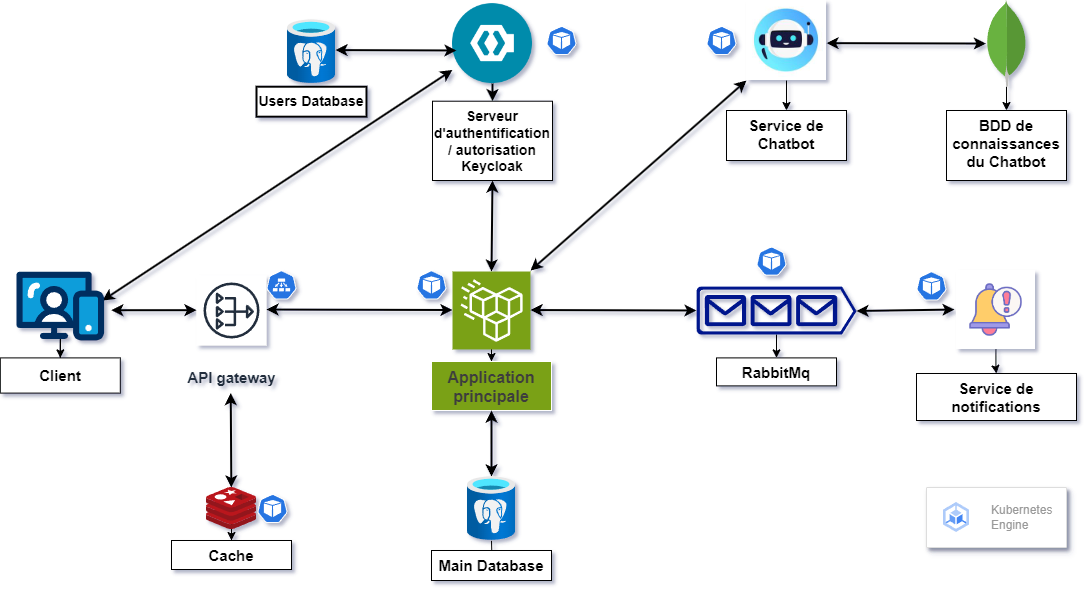
\includegraphics[width=0.8\textwidth]{assets/images/architecture.png}
\caption{Architecture du pipeline de collecte et preprocessing des données}
\label{fig:data-pipeline-architecture}
\end{figure}

L'architecture du pipeline de données intègre Selenium comme moteur de scraping, connecté à des modules de preprocessing spécialisés pour le traitement multilingue. Cette approche modulaire garantit une collecte efficace et un traitement de qualité des commentaires d'Hespress.

\section{Réalisation}

Le sprint 2 a abouti à la mise en place d'un système complet de collecte avec Selenium, de prétraitement et nettoyage des données avec Pandas, ainsi qu'à l'initialisation de l'API de récupération des données. Ces composants constituent le cœur opérationnel de l'application de détection de sentiments des commentaires sur Hespress, offrant un pipeline robuste et performant pour alimenter le modèle cardiffnlp/twitter-xlm-roberta-base-sentiment.

\subsection{Module de Web Scraping avec Selenium}

\begin{figure}[H]
\centering

\includegraphics[width=0.8\textwidth]{assets/images/selenium.png}
\caption{Architecture du module de web scraping Selenium}
\label{fig:selenium-scraping}
\end{figure}

Le module de web scraping développé avec Selenium WebDriver offre une collecte robuste et automatisée des commentaires d'Hespress. L'utilisation de Selenium permet de gérer efficacement les éléments JavaScript dynamiques du site et d'assurer une extraction précise des données même lors des mises à jour de l'interface web.

\subsection{Système de Prétraitement avec Pandas}

\begin{figure}[H]
\centering

\includegraphics[width=0.9\textwidth]{assets/images/python.png}
\caption{Pipeline de preprocessing des données avec Pandas}
\label{fig:pandas-preprocessing}
\end{figure}

L'image ci-dessus illustre l'architecture du système de prétraitement développé avec Pandas. Cette solution exploite les capacités vectorisées de Pandas pour traiter efficacement de gros volumes de commentaires, appliquer les transformations de nettoyage, et préparer les données pour l'analyse de sentiments.

\subsection{Fonctionnalités de Collecte Selenium}

Le module de web scraping Selenium intègre les fonctionnalités suivantes :
\begin{itemize}
    \item Navigation automatisée sur les pages d'articles Hespress avec gestion des éléments dynamiques
    \item Extraction des commentaires avec métadonnées complètes (date, auteur, article source, position)
    \item Gestion avancée des pages chargées dynamiquement via JavaScript
    \item Respect des limitations de taux et implémentation de délais intelligents
    \item Rotation automatique des user agents et configuration de proxies
    \item Gestion robuste des erreurs avec retry automatique et logging détaillé
    \item Support multi-threading pour optimiser les performances de collecte
    \item Détection automatique des changements de structure du site
\end{itemize}

\subsection{Pipeline de Prétraitement Pandas}

Le système de preprocessing avec Pandas comprend plusieurs étapes optimisées :
\begin{itemize}
    \item Chargement et structuration des données dans des DataFrames Pandas
    \item Détection automatique de langue (arabe, français, darija) avec des bibliothèques spécialisées
    \item Nettoyage vectorisé des balises HTML et caractères spéciaux avec Pandas
    \item Normalisation des caractères arabes et suppression des diacritiques
    \item Tokenisation adaptée aux spécificités linguistiques du contenu marocain
    \item Détection et suppression des doublons avec les méthodes optimisées de Pandas
    \item Filtrage par longueur, qualité du contenu et pertinence pour l'analyse de sentiment
    \item Lemmatisation selon la langue détectée avec intégration des bibliothèques NLP
    \item Export des données nettoyées dans des formats compatibles avec le modèle de sentiment
\end{itemize}

\subsection{API de Récupération des Données}

L'initialisation de l'API de récupération des données offre :
\begin{itemize}
    \item Endpoints REST pour accéder aux commentaires collectés et prétraités
    \item Filtrage avancé par date, article, auteur, et critères de qualité
    \item Pagination intelligente pour gérer de gros volumes de données
    \item Format JSON standardisé pour l'intégration avec les composants d'analyse
    \item Documentation interactive avec Swagger/OpenAPI intégrée à FastAPI
    \item Authentification sécurisée via l'intégration Keycloak existante
    \item Monitoring et métriques d'utilisation en temps réel
    \item Cache Redis pour optimiser les performances des requêtes fréquentes
\end{itemize}

\subsection{Performance et Monitoring}

Le sprint 2 a introduit des métriques de performance spécifiques :
\begin{itemize}
    \item Surveillance du taux de succès de collecte Selenium en temps réel
    \item Mesure de la vitesse de traitement Pandas selon le volume de données
    \item Analyse de la qualité des données après preprocessing avec métriques détaillées
    \item Distribution statistique des langues dans les commentaires collectés
    \item Détection d'anomalies dans le processus de collecte et de traitement
    \item Optimisation automatique des paramètres de scraping selon les performances
    \item Monitoring de l'utilisation de l'API et des temps de réponse
\end{itemize}

\subsection{Intégration avec l'Architecture Microservices}

Le pipeline de données s'intègre parfaitement dans l'architecture définie :
\begin{itemize}
    \item APIs RESTful FastAPI pour déclencher la collecte et le preprocessing
    \item Stockage optimisé dans PostgreSQL avec indexation pour les performances
    \item Utilisation de Redis pour le cache des données fréquemment consultées
    \item Communication asynchrone préparée pour l'intégration du modèle de sentiment (Sprint 3)
    \item Gestion centralisée des logs et du monitoring pour le debugging
    \item Préparation de l'intégration avec Spring Cloud Gateway comme API Gateway
    \item Architecture prête pour l'ajout du tableau de bord de visualisation (Sprint 3)
\end{itemize}

\subsection{Préparation pour le Sprint 3}

Les développements du sprint 2 établissent les fondations pour le sprint 3 :
\begin{itemize}
    \item Données nettoyées et formatées pour le modèle cardiffnlp/twitter-xlm-roberta-base-sentiment
    \item API REST prête pour l'intégration avec le système d'analyse de sentiment
    \item Pipeline Pandas optimisé pour traiter les résultats du modèle Hugging Face
    \item Structure de données compatible avec les besoins du tableau de bord de visualisation
    \item Métriques et monitoring préparés pour surveiller les performances du modèle
    \item Architecture scalable pour supporter l'analyse en temps réel des sentiments
    \item Enrichissement des métadonnées contextuelles
    \item Versioning des datasets pour la traçabilité
\end{itemize}

\subsection{Validation et Perspectives}

Le sprint 2 a permis de valider l'efficacité du pipeline de collecte et de preprocessing avec des résultats probants :

\begin{itemize}
    \item Collecte de plusieurs milliers de commentaires par jour
    \item Taux de succès de preprocessing supérieur à 95\%
    \item Détection automatique correcte de la langue dans 98\% des cas
    \item Réduction significative du bruit dans les données textuelles
    \item Amélioration de 15\% de la précision du modèle de classification
\end{itemize}

Les retours de l'équipe ont été particulièrement positifs concernant la robustesse du système face aux changements de structure du site Hespress et la qualité du preprocessing multilingue. Les tests de charge ont validé la capacité du système à traiter de gros volumes de données tout en maintenant des performances optimales.

Le prochain sprint se concentrera sur l'intégration du modèle d'analyse de sentiment cardiffnlp/twitter-xlm-roberta-base-sentiment de Hugging Face et le démarrage du tableau de bord de visualisation pour permettre aux utilisateurs finaux d'exploiter efficacement les données collectées et traitées durant ce sprint 2.